%% fancy header & foot
\pagestyle{fancy}
\lhead{[ELEC-H-2001] Électricité\\ Séance \no 10 : Séance récapitulative - Théorie des circuits \ifthenelse{\boolean{corrige}}{~-- corrigé}{}}
\rhead{v1.0.0\\ page \thepage}
\cfoot{}
%%

\pdfinfo{
/Author (Renaud Theunissen et Youssef Agram, ULB -- BEAMS-EE)
/Title (Séance 10 ELEC-H-2001, Séance récapitulative - Théorie des circuits)
/ModDate (D:\pdfdate)
}

\hypersetup{
pdftitle={Séance 10 [ELEC-H-2001] Électricité : Séance 11 ELEC-H-2001, Séance récapitulative - Théorie des circuits},
pdfauthor={Renaud Theunissen et Youssef Agram, ©2020 ULB - BEAMS-EE},}

\setlength{\parskip}{0.5cm plus4mm minus3mm} %espacement entre §
\setlength{\parindent}{0pt}


\begin{document}
\long\def\nothx/*#1*/{}
\tptitle{}{Séance 10~: Séance récapitulative - Théorie des circuits}
\section{But de la séance}
L'objectif de cette séance est de vous proposer des questions pratique typiques d'examen pour la partie théorie des circuits.
Cette séance sert de synthèse aux séances d'exercices consacrées aux circuits.

\section{Pré-requis}
Avant la séance, vous aurez relu les chapitres et sections suivants:
\begin{itemize}
	\item Chapitre 1 - Circuits à éléments concentrés
		\begin{itemize}
		\item Section 1.6 - Puissance instantanée, conventions et passivité
		\end{itemize}
	\item Chapitre 2 - Dipôles idéaux
	    \begin{itemize}
	        \item Section 2.2 - Dipôles réels >< Dipôles idéaux
	        \item Section 2.3 - Charges idéales : trois effets physiques
	        \item Section 2.6 - Sources idéales
	    \end{itemize}
	\item Chapitre 4 - Équivalence de Thévenin et adaptation d'impédance
		\begin{itemize}
		\item Section 4.1 - Circuits équivalents et théorèmes de Thévenin et Norton
		\item Section 4.2 - Impédance d'entrée, impédance de sortie (et fem à vide)
		\item Section 4.3 - Adaptation d'impédance
		\end{itemize}
	\item Chapitre 5 - Résoudre un circuit : procédure de base et accélérateurs
	    \begin{itemize}
	        \item Section 5.1 - Vocabulaire lié aux circuits 
	        \item Section 5.2 - Lois de Kirchhoff
	        \item Section 5.3 - Procédure canonique en 6 étapes
	        \item Section 5.4 - Illustration : Diviseur résistif (étendu aux impédances)
	        \item Section 5.5 - Équivalences série et parallèle
	        \item Section 5.6 - Utilisation des théorèmes de Thévenin et Norton pour résoudre un circuit
	        \item Section 5.8 - Théorème de superposition
	    \end{itemize}
	\item Chapitre 6 - Résoudre un circuit réactif dans le domaine temporel
	    \begin{itemize}
	        \item Section 6.1 - Éléments réactifs : Rappels 
		    \item Section 6.2 - Analyse temporelle du circuit RC (source en échelons)
		    \item Section 6.3 - Analyse temporelle du circuit RL (source en échelons)
		    \item Section 6.5 - Analyse temporelle du circuit RL (source sinusoïdale avec échelon)
		    \item Section 6.6 - Analyse temporelle du circuit RLC
	    \end{itemize}
	\item Chapitre 7 - Résoudre un circuit réactif dans le domaine fréquentiel
	    \begin{itemize}
	        \item Section 7.3 - Phaseurs
		    \item Section 7.4 - Impédances et admittances
	    \end{itemize}
\end{itemize}

\vspace{5pt}

\newpage

\section{Théorie des circuits - Exercices d'examens}
\subsection{Examen Juin 2016 (Q4)}

Soit le circuit suivant \\

\begin{figure}[h!]
    \centering
    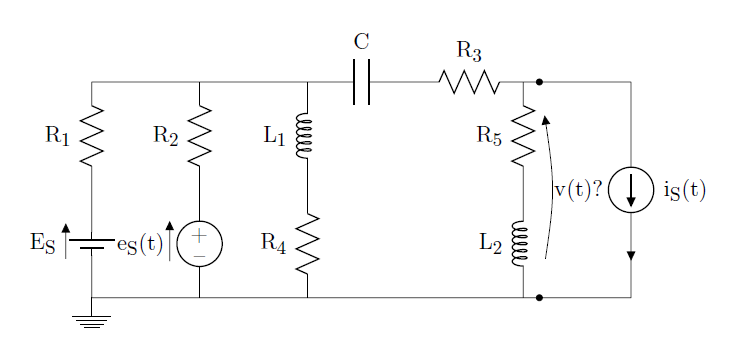
\includegraphics[width = 17cm]{TpQEx_Circuits/Q4_Juin_2016.PNG}
    %\caption{}
    \label{fig:Q4_TheoCircuitsJuin2016}
\end{figure}
Où les sources sont $E_S = E_1$, $e_{S}(t) = E_1 +E_2*sin(\omega_1 t)$ et $i_s(t) = I * (1+cos(\omega_2 t+\Phi)$. 
Les valeurs des différents paramètres sont les suivantes :
\begin{figure}[h!]
    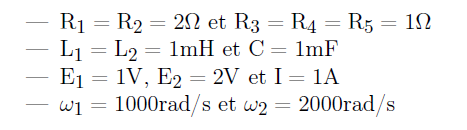
\includegraphics[width = 10cm]{TpQEx_Circuits/Q4_Juin_2016_HINT.PNG}
    %\caption{}
    \label{fig:Q4_TheoCircuitsJuin2016_HINT}
\end{figure}

\Question{
\newline
On vous demande de déterminer la tension v(t) en suivant les indications suivantes :
\begin{enumerate}
    \item Suivez la procédure canonique
    \item Expliquez votre démarche et mettez en évidence les étapes qui vous sont nécessaires pour trouver les résultats intermédiaires
    \item Utilisez au minimum une fois un équivalent de Thévenin en expliquant en quoi cette méthode vous permet de faciliter la résolution de ce circuit
    \item Vous ne devez pas développer les racines et arctangentes jusqu’au bout. Par exemple, si vous tombez sur $\sqrt{7^2+11^2}$ ou $Arg(7+11j)$, notez respectivement $\sqrt{170}$ ou $arctg(\dfrac{11}{7})$ (pas de valeurs avec décimales)
\end{enumerate}
}
{En utilisant le théorème de superposition\\
$E_S$ : la capa se comporte comme un circuit ouvert –> $V_1 = 0V$\\
\textbf{Composante continue} de $e_s(t)$ : Idem –> $V_2 = 0V$\\
\textbf{Composante continue} de $i_S(t)$ : $V_3$ = $- R_5 * I = – 1V$\\
$E_2sin(\omega_1t)$ : Thévenin
\begin{equation*}
    Z_1 = R_1 (R_4+j\omega_1L_1) \implies Z_1 = \dfrac{2+2j}{3+j}
\end{equation*}
\begin{equation*}
    Z_2=R_3+\dfrac{1}{j\omega_1C} \implies Z_2 = 1–j
\end{equation*}
\begin{equation*}
    Z_3 = R_5+j\omega_1L_2 \implies Z_3=1+j
\end{equation*}
\begin{equation*}
    Z_{Th} = Z_2 + R_2
\end{equation*}
\begin{equation*}
    Z_1 = 1 – j + \dfrac{1+j}{2+j} \implies Z_1 = \dfrac{4}{2+j}
\end{equation*}
\begin{equation*}
    \underline{V}_{Th} = \dfrac{Z_1}{R_2+Z_1} \underline{E}_S \implies \underline{V}_{Th}= \dfrac{1+j}{4+2j}\underline{E}_S
\end{equation*}
\begin{equation*}
    \underline{V}_4 = \dfrac{Z_3}{Z_3+Z_{Th}} \implies \underline{V}_4=\dfrac{-1+2j}{7+11j}\underline{E}_S
\end{equation*}
\begin{equation*}
    v_4(t) = \dfrac{2\sqrt{5}}{\sqrt{170}}sin(1000t - arctan(2)-acrtan\left(\dfrac{11}{7}\right)
\end{equation*}

$I*cos(\omega_2t + \Phi)$ : Thévenin
\begin{equation*}
    Z_A = R_1//R_2//(R_4 + j\omega_4*L_1) = \dfrac{1+2j}{2+2j}
\end{equation*}
\begin{equation*}
    Z_B = R_3 + \dfrac{1}{j\omega_2*C}=1-0,5j
\end{equation*}
\begin{equation*}
    Z_3= R_5 +j\omega_2*L_2 = 1+2j
\end{equation*}
\begin{equation*}
    Z_{eq} = (Z_A + Z_B)//Z_3 = \dfrac{-2+11j}{2+9j}
\end{equation*}
\begin{equation*}
    \underline{V}_5 = -Z_{eq}*\underline{I}_S = \dfrac{2-11j}{2+9j}*e^{\Phi} 
\end{equation*}
\begin{equation*}
    \underline{V}_{5} = \dfrac{5*\sqrt{5}}{\sqrt{85}}*e^{j*\left(\Phi + arctan(\dfrac{11}{2}) - arctan(\dfrac{9}{2})\right)}
\end{equation*}
\begin{equation*}
    v_5(t) = \dfrac{5*\sqrt{5}}{\sqrt{85}}*cos\left(2000*t+\Phi+ arctan(\dfrac{11}{2}) - arctan(\dfrac{9}{2})\right)
\end{equation*}

On trouve ainsi\\
\begin{equation*}
    v(t) = V_1 + V_2 + V_3 + v_4(t) + v_5(t)

    v(t) = –1 + \dfrac{2}{\sqrt{170}}*sin\left(1000*t - arctan(\dfrac{11}{7})\right) - \dfrac{\sqrt{125}}{\sqrt{80}}*cos\left(2000*t+\Phi-arctan(2) - arctan(\dfrac{3}{2})\right)
\end{equation*}

}

\newpage
\subsection{Examen Janvier 2014 (Q3)}
Soit le circuit suivant :

\begin{figure}[h!]
    \centering
    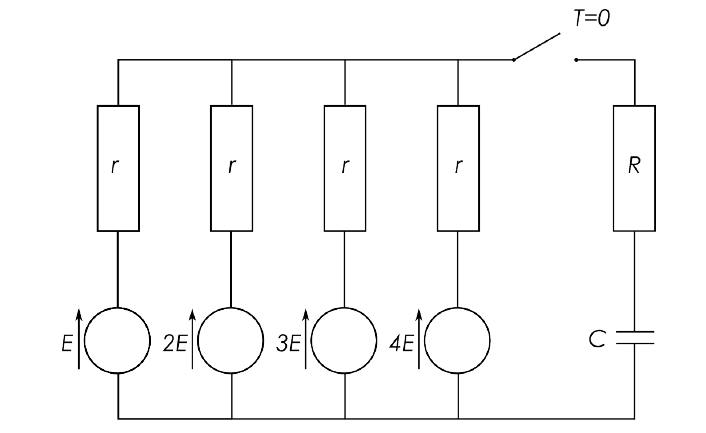
\includegraphics[width = 11cm]{TpQEx_Circuits/Q3_Janv_2014.PNG}
    %\caption{}
    \label{fig:Q3_TheoCircuitsJanv2014}
\end{figure}
Où $E = 20V$, $r = 4\Omega$,$R = 1\Omega$ et $C = 0,1 F$.
Avant $t = 0$, l'interrupteur est ouvert. On ferme l'interrupteur à l'instant $t = 0$. La charge initiale de la capacité est nulle.
Après une prise de mesure, on a relevé les deux courbes suivantes (temps [s] en abscisse et courant [A] ou tension [V] en ordonnée).
\begin{figure}[h!!]
    \centering
    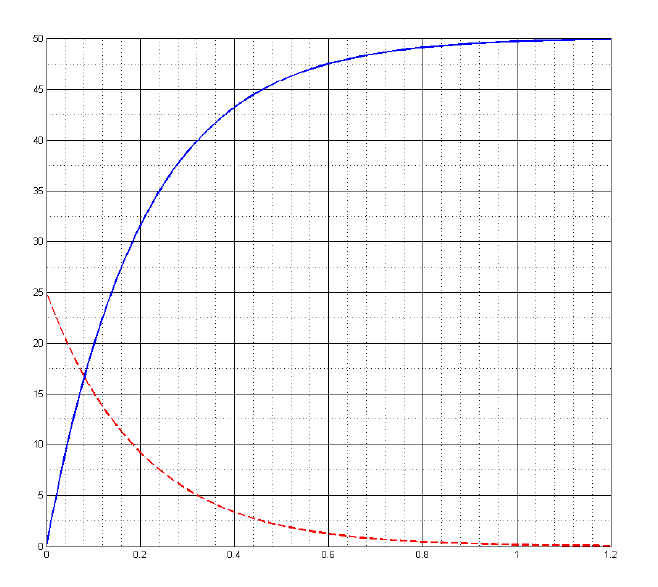
\includegraphics[width = 12cm]{TpQEx_Circuits/Q3_Janv_2014_Graph.PNG}
    %\caption{}
    \label{fig:Q3_TheoCircuitsJanv2014_Graph}
\end{figure}

\begin{itemize}
    \item \Question{Identifiez l’élément du schéma (source(s), capacité, resistance(s)) auquel se rapportent ces deux graphes.
    }
    {
    Ici l'élément dont il est question est un condensateur.
    }
    \item \Question{Identifiez la grandeur (tension(s) ou courant(s)) présente sur l’ordonnée pour chaque courbe (trait continu et trait discontinu).
    }
    {
    \textbf{Trait continu} :\\
    Cette courbe représente la tensions aux bornes du condensateur $v_C(t)$.\\
    \textbf{Trait discontinu} :\\
    Cette courbe re présente l'intensité du courant traversant le condensateur $i_C(t)$.
    }
    \item \Question{Sur base de ce graphique, déterminer la valeur de la constante de temps $\tau$ du circuit.
    }
    {
    La constante de temps $\tau$ est par définition le temps nécessaire à la tension aux bornes du condensateur pour atteindre 63\% de sa valeur de régime :
    \begin{equation*}
        v_C(\tau) = v_C(\infty) *(1-\exp{-1})\approx 0,63*v_C(\infty)
    \end{equation*}
    Graphiquement, il suffit de tracer une ligne horizontale passant par $0,63*50 = 31,5V$.\\
    L'intersection avec le graphique de $v_C(t)$ donne $\tau = 0,2s$.
    }
    \newpage\item \Question{Déterminez les paramètres $R_{th}$ et $V_{th}$ de l’équivalent de Thévenin du circuit vu aux bornes du condensateur.
    }
    {
    \begin{itemize}
        \item Pour $R_{Th}$ :\\
        Pour trouver la résistance équivalente de Thévenin, il faut court-circuiter les sources du circuit.
        Par les propriétés de la mise en parallèle et de la mise en série des résistances on trouve : 
        \begin{equation*}
            R_{Th} = R + (r//r//r//r)\implies R_{Th}=R+\dfrac{r}{4}
        \end{equation*}
        \begin{figure}[h!!!]
            \centering
            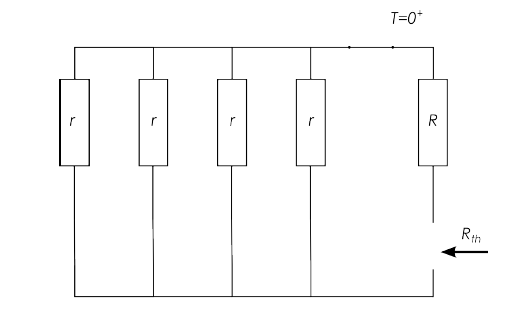
\includegraphics[width = 10cm]{TpQEx_Circuits/TP11Q2_Reso1.PNG}
    %\caption{}
            \label{fig:Q3_TheoCircuitsJanv2014_Reso1}
        \end{figure}
        \item Pour $V_{Th}$ :\\
        Pour trouver la tension équivalente de Thévenin, on doit résoudre le circuit à vide (remplacer le condensateur par un circuit ouvert). Le courant passant par la branche de droite sera alors nul et il n'y a pas de chute de potentiel dans la résistance $R$ (car $V_R = R*i = 0$).
        \begin{figure}[h!!!!]
            \centering
            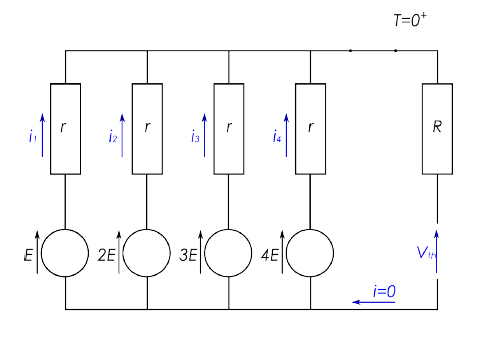
\includegraphics[width = 10cm]{TpQEx_Circuits/TP11Q2_Reso2.PNG}
    %\caption{}
            \label{fig:Q3_TheoCircuitsJanv2014_Reso2}
        \end{figure}
        \item \textbf{Résolution 1 - Lois de Kirchhoff}\\
        Soit $i_k(t)$ le courant passant dans la $k^{ième}$ branche (de gauche à droite).
        La mise en parallèle des cinq branches nous permet d'égaler les tensions :
        \begin{equation*}
            V_{Th} = E - r_{i_1} = 2E - r_{i_2} = 3E - r_{i_3} = 4E - r_{i_4}
        \end{equation*}
        Par la loi des noeuds, on a donc :
        \begin{equation*}
            i(t) = \sum^4_{k=1}\left(i_k(t)\right) = 0
            
            \iff i_1+i_1+\dfrac{E}{r}+i_1\dfrac{2E}{r}+i_1\dfrac{3E}{r} = 4i_1+6\dfrac{E}{r} = 0
            
            \iff i_1 = \dfrac{-3}{2}\dfrac{E}{r}
            
        \end{equation*}
        Et donc finalement : $V_{Th}=E-r*i_1 = \dfrac{5}{2}*E$
        \item \textbf{Résolution 2 - Théorème de superposition}\\
        Soit $E_i(i = 1,2,3,4)$ les 4 sources et $V_{Th_i}$les contributions de chacune d'elle à la tension de Thévenin.\\
        On annule donc toutes les sources sauf $E_i$ pour les 4 cas (i=1,2,3,4), on calcule chacune des contributions puis on les somme pour avoir $V_{Th}$.\\
        \textit{Remarque}\\
        Beaucoup d'entre vous 
    \end{itemize}
    }
\end{itemize}

\newpage
\subsection{Examen Janvier 2015 (Q1.3)}
Soit le circuit suivant avec :
\begin{itemize}
    \item $E_S$ une source de tension continue d'amplitude $E$
    \item 7 résistances de même valeur $R$
    \item Un condensateur $C$
\end{itemize}
\begin{figure}[h!]
    \centering
    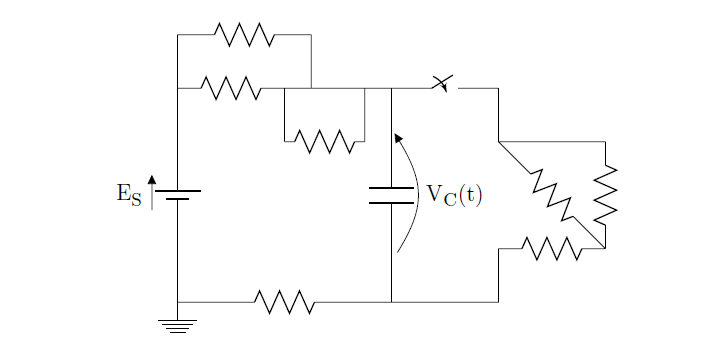
\includegraphics[width = 14cm]{TpQEx_Circuits/Q1_3_Janv_2015.PNG}
    %\caption{}
    \label{fig:Q1_3_TheoCircuits_Janv2015}
\end{figure}
On ferme l'interrupteur à l'instant $t=0$.\\
Quelle est l'expression analytique de $V_C(t)$ pour tout temps $t$?


\newpage
\subsection{Examen Septembre 2015 (Q4)}

\begin{figure}[h!]
    \centering
    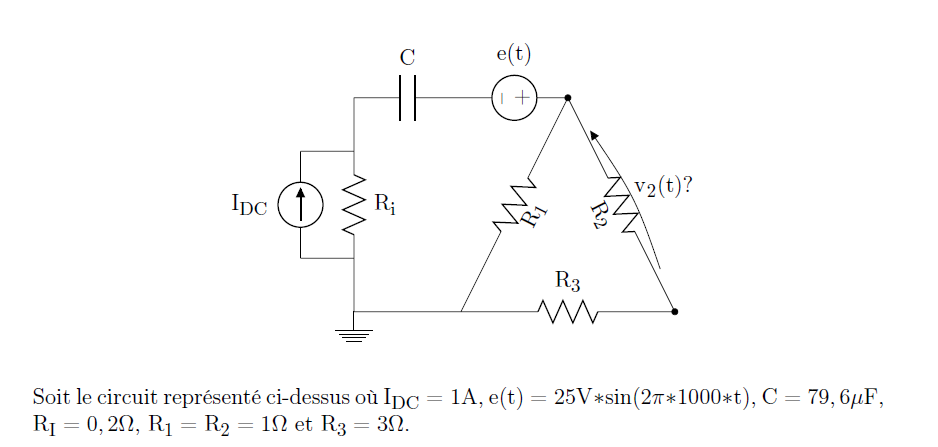
\includegraphics[width = 17cm]{TpQEx_Circuits/Q4_Sept_2015.PNG}
    %\caption{}
    \label{fig:Q4_TheoCircuitsSept2015}
\end{figure}
Que vaut $V_2$, l'amplitude de $v_2(t)$ pour tout temps $t$?

\newpage

\subsection{Examen Septembre 2019 (Q1) Modifiée}

\begin{figure}[h!]
    \centering
    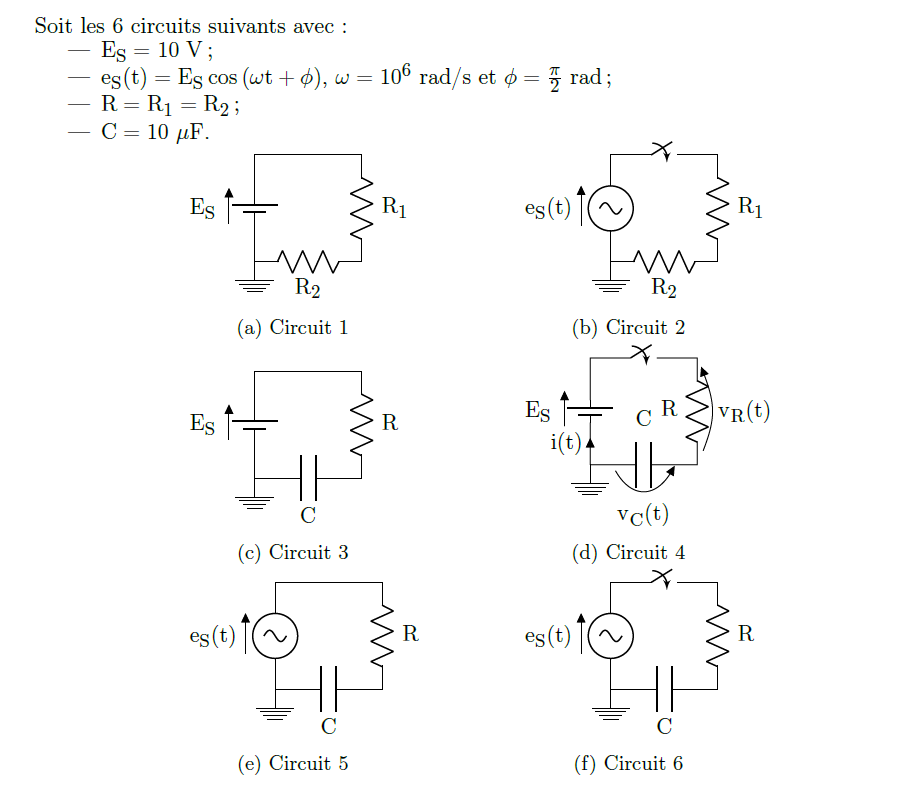
\includegraphics[width = 17cm]{TpQEx_Circuits/Q1_Sept_2019.PNG}
    %\caption{}
    \label{fig:Q1_TheoCircuitsSept2019}
\end{figure}


\begin{enumerate}
    \item Pour quels circuits devrions-nous utiliser les phaseurs \textbf{uniquement} pour résoudre le circuit?
    \item Pour quels circuits devrions-nous utiliser les lois long terme \textbf{uniquement} pour résoudre le circuit?
    \item Pour quels circuits la méthode des phaseurs ne suffira pas à résoudre le circuit?
    \item Déterminez la tension aux bornes du condensateur pour les circuits 3 à 6 et pour tout temps.
    \item Déterminez la tension aux bornes de la résistance $R_1$ des circuits 1 et 2, pour tous temps t
\end{enumerate}

\newpage
\subsection{Examen Septembre 2019 (Q2)}

Soit le circuit suivant comportant :
\begin{itemize}
    \item Une source de tension sinusoïdale : $e_1(t) = E_1 sin(\omega t)$
    \item Une deuxième source de tension sinusoïdale : $e_2(t) = E_2 sin(\omega t+\alpha)$
    \item Une source de courant continu : $I_S$
    \item 4 résistances de même valeur : $R_1$,$R_2$,$R_3$ et $R_4$
    \item Un condensateur $C$ et une inductance $L$
\end{itemize}
\begin{figure}[h!]
    \centering
    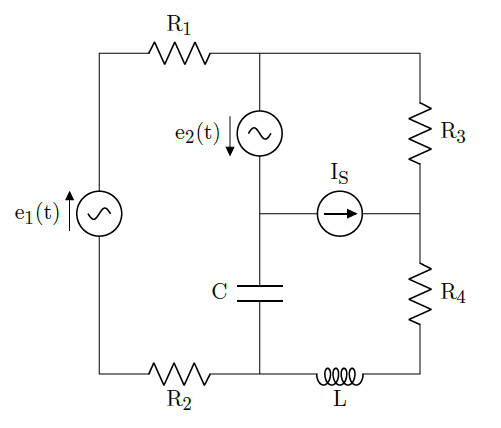
\includegraphics[width = 14cm]{TpQEx_Circuits/Q2_Sept_2019.PNG}
    %\caption{}
    \label{fig:Q2_TheoCircuitsSept2019}
\end{figure}

En utilisant les principes et théorèmes vus au cours, déterminez l'équivalent de Thévenin de ce circuit vu par la résistance $R_4$ de la manière la plus efficace possible.
\end{document}